\documentclass{BHCexam}
%\usepackage[colorlinks,linkcolor=black]{hyperref}
\usepackage{yhmath}
\begin{document}
\biaoti{压轴题复习}
\fubiaoti{ }
\maketitle
\tableofcontents
\section{选择}
\begin{questions}
\qs 如果,函数$f(x)$的图象为折线$ ACB $,则不等式$ f(x)\ge \log_2(x+1) $的解集是\xx
\begin{center}
\begin{tikzpicture}
\draw[->] (-2,0)--(3,0) node[below]{$x$};
\draw[->] (0,-1)--(0,2.8) node[left]{$y$};
\draw (-1,0)--(0,2)--(2,0);
\node [above left](A) at (-1,0){$A$} ;
\node [above right](B) at (2,0){$B$} ;
\node [above right](C) at (0,2){$C$} ;
\node [below left](O) at (0,0){$O$} ;
\node [below ](A1) at (-1,0){$-1$} ;
\node [below](B1) at (2,0){$2$} ;
\node [above left](C1) at (0,2){$2$} ;
\end{tikzpicture}
\end{center}
\vspace{-2em}
\twoch{$ \left\{\ x\ \left|-1<x\le0 \right.\right\}$}{$ \left\{\ x\ \left|-1\le x\le 1\right.\right\} $}{$ \left\{\ x\ \left|-1 < x\le1\right.\right\} $}{$ \left\{\ x\ \left|-1 \le x\le2\right.\right\} $}
\qs 设$ A(0,0),~B(4,0),~C(t+4,4),~D(t,4)~(t\inR) $.记$ N(t) $为平行四边形$ ABCD $内部(不含边界)的整数点的个数,其中整数点是指横、纵坐标都是整数的点,则函数$ N(t) $的值域为\xx
\onech{$ \left\{9,10,11\right\}$}{$\left\{9,10,12\right\} $}{$\left\{9,11,12\right\} $}{$\left\{10,11,12\right\} $}
\qs 直线$ l:ax+\dfrac{1}{a}y-1=0 $与$x,~y$轴的交点分别为$ A,~B $,直线$ l $与圆$ O:~x^2+y^2=1 $的交点为$ C,~D .$给出下面三个结论:\\
\ding{192} $ \forall a\ge 1,S_{\triangle AOB}=\dfrac{1}{2} $;\\
\ding{193} $\exists a\ge1,\abs{AB}<\abs{CD}$;\\
\ding{194} $\exists a\ge 1,S_{\triangle COD}<\dfrac{1}{2}$.\\
则所有正确结论的序号是\xx
\onech{\ding{192}\ding{193}}{\ding{193}\ding{194}}{\ding{192}\ding{194}}{\ding{192}\ding{193}\ding{194}} 
\qs 已知$ A(0,1),~ $点$ B $在曲线$ G:y=\ln (x+1) $上,若线段$ AB $与曲线$ M:y=\dfrac{1}{x} $相交且交点恰为线段$ AB $的中点,则称$ B $为曲线$ G $关于曲线$ M $的一个关联点.记曲线$ G $关于曲线$ M $的关联点的个数为$ a $,则\xx
\onech{$ a=0$}{$ a=1$}{$ a=2$}{$ a>2$}
\qs 已知圆$ C:(x-3)^2+(y-4)^2=1 $和两点$ A(-m,0),B(m,0)~(m>0) $,若圆上存在点$ P $,使得$ \angle APB=90^{\circ} $,则$ m $的最大值为\xx
\onech{$7$}{$6$}{$5$}{$4$}
\qs 设点$ M(x_0,1),~ $若在圆$ O: x^2+y^2=1 $上存在点$ N $,使得$ \angle OMN=45^{\circ} $,则$ x_0 $的取值范围是\xx
\onech{$ \left[-1,1\right]$}{$ \left[-\dfrac{1}{2},\dfrac{1}{2}\right]$}{$\left[-\sqrt{2},\sqrt{2}\right] $}{$ \left[-\dfrac{\sqrt{2}}{2},\dfrac{\sqrt{2}}{2}\right]$}
\qs 设直线$ l:~3x+4y+a=0,~ $圆$ C:(x-2)^2+y^2=2 $,若在圆$ C $上存在两点$ P,~Q,~ $在直线$ l $上存在一点$ M $,使得$ \angle PMQ =90^{\circ}$,则$ a $的取值范围是\xx
\twoch{$ \left[-18,6\right]$}{$ \left[6-5\sqrt{2},6+5\sqrt{2}\right]$}{$ \left[-16,4\right]$}{$ \left[-6-5\sqrt{2},-6+5\sqrt{2}\right]$}
\qs 已知函数$f(x)=x^3-6x^2+9x-abc,~a<b<c,~$且$ f(a)=f(b)=f(c)=0 ,~$给出如下结论:\\
\ding{192} $ f(0)f(1)>0 ;$\quad \ding{193}$f(0)f(1)<0;$\quad \ding{194}$f(0)f(3)>0;$\quad \ding{195}$f(0)f(3)<0;$\\
其中正确的结论的序号是\xx
\onech{\ding{192}\ding{194}}{\ding{192}\ding{195}}{\ding{193}\ding{194}}{\ding{193}\ding{195}}
\qs 已知函数$f(x)=\dfrac{\bm{e}^x-\bm{e}^{-x}}{2},x\inR$,若对任意$ \theta\in\left(0,\dfrac{\pi}{2}\right] $,都有$ f(m\sin \theta)+f(1-m)>0 $成立,则实数$ m $的取值范围是\xx
\onech{$ \left(0,1\right)$}{$ \left(0,2\right)$}{$ \left(-\infty,1\right)$}{$ \left(-\infty,1\right]$}
\qs 已知函数$f(x)=2mx^2-2(4-m)x+1,~g(x)=mx$,若对于任意实数$ x ,f(x)$与$g(x)$的值至少有一个为正数,则实数$ m $的取值范围是\xx
\onech{$ \left(0,2\right)$}{$ \left(0,8\right)$}{$ \left(2,8\right)$}{$ \left(-\infty,0\right)$}
\question
设函数$f(x)=e^x(2x-1)-ax+a$,其中$a<1$,若存在唯一的整数$x_0$使得$f(x_0)<0$,则$a$的取值范围是\xx
\twoch{$\Big[-\dfrac{3}{2e},1\Big)$}{$\Big[-\dfrac{3}{2e},\dfrac{3}{4}\Big)$}{$\Big[\dfrac{3}{2e},\dfrac{3}{4}\Big)$}{$\Big[\dfrac{3}{2e},1\Big)$}
\question
已知函数$f(x)=\Bigg\{\begin{aligned}
&-x^2+2x,&x\le0,\\
&\ln(x+1),&x>0.
\end{aligned}$若$\abs{f(x)}\ge ax$,则$a$的取值范围是\xx
\onech{$\left(-\infty,0\right]$}{$\left(-\infty,1\right]$}{$\left[-2,-1\right]$}{$\left[-2,0\right]$}
\qs 已知函数$f(x)=\Bigg\{\begin{aligned}
&\left|\log_4x\right|,&0<x\le 4,\\&x^2-10x+25,&x>4.
\end{aligned}$若$ a,~b,~c,~d $是互不相同的正数,且$ f(a)=f(b)=f(c)=f(d),~ $则$ abcd $的取值范围是\xx
\onech{$ \left(24,25\right) $}{$ \left(18,24\right) $}{$ \left(21,24\right) $}{$ \left(18,25\right) $}
\qs 已知函数$f(x)=\Bigg\{\begin{aligned}
&\abs{\lg x},&0<x\le10 \\
&-\dfrac{1}{2}x+6,&x>10.
\end{aligned}$若$ a,b,c $互不相等,且$ f(a)=f(b)=f(c) $,则$ abc $的取值范围是\xx
\twoch{$ \left(1,10\right)$}{$ \left(5,6\right)$}{$ \left(10,12\right)$}{$ \left(20,24\right)$}
\qs 已知函数$f(x)=\Bigg\{\begin{aligned}
&-x^2+4x,&x\le 4,\\
&\log_2x,&x>4.
\end{aligned}$若$y=f(x)$在区间$ \left(a,a+1\right) $上单调递增,则实数$ a $的取值范围是\xx
\fourch{$ \left(-\infty,1\right] $}{$ \left[1,4\right] $} {$ \left[4,+\infty\right) $}{$ \left(-\infty,1\right]\cup\left[4,+\infty\right) $}
\qs 已知函数$f(x)$在$ \left[0,+\infty\right) $上是增函数,$ g(x)=f\left(\abs{x}\right) >g(1)$,则$ x $的取值范围是\xx
\twoch{$ \left(0,10\right) $}{$ \left(10,+\infty\right) $}{$ \left(\dfrac{1}{10},10\right) $}{$ \left(0,\dfrac{1}{10}\right)\cup\left(10,+\infty\right) $}
\qs 已知函数$f(x)=\sin (\omega x-\dfrac{\pi}{3})$,~点$ A(m,~n) $,~$ B(m+\pi,~n) (\left|n\right|\ne 1)$都在曲线$ y=f(x) $上,且线段$ AB $与曲线$ y=f(x) $有五个公共点,则$ \omega $的值为\xx
\onech{$ 4 $}{$ 2 $}{$ \dfrac{1}{2} $}{$ \dfrac{1}{4} $}
\qs 将函数$ y=\sin\left(2x+\dfrac{\pi}{3}\right) $图象上的点$ P\left(\dfrac{\pi}{4},t\right) $向左平移$ s~(s>0) $个单位长度得到点$ P' $.若$ P' $位于函数 $ y=\sin 2x $的图象上,则\xx
\twoch{$ t=\dfrac{1}{2},~s\text{的最小值为}\dfrac{\pi}{6} $}{$ t=\dfrac{\sqrt{3}}{2},~s\text{的最小值为}\dfrac{\pi}{6} $}{$ t=\dfrac{1}{2},~s\text{的最小值为}\dfrac{\pi}{3} $}{$ t=\dfrac{\sqrt{3}}{2},~s\text{的最小值为}\dfrac{\pi}{3} $}
\qs 将函数$ y=\sin (2x+\dfrac{\pi}{6}) $的图象向左平移$ m~(m>0) $个单位长度,得到函数$ y=f(x) $图象在区间$ \left[-\dfrac{\pi}{12},\dfrac{5\pi}{12}\right] $上单调递减,则$ m $的最小值为\xx
\onech{$ \dfrac{\pi}{12} $}{$ \dfrac{\pi}{6} $}{$ \dfrac{\pi}{4} $}{$ \dfrac{\pi}{3} $}
\qs 已知函数$f(x)=\Bigg\{\begin{aligned}
\sin(x+a),x\le 0\\\cos (x+b),x>0
\end{aligned}$是偶函数,则下列结论可能成立的是\xx
\twoch{$ a=\dfrac{\pi}{4},b=-\dfrac{\pi}{4}$}{$ a=\dfrac{2\pi}{3},b=\dfrac{\pi}{6}$}{$a=\dfrac{\pi}{3},b=\dfrac{\pi}{6} $}{$ a=\dfrac{5\pi}{6},b=\dfrac{2\pi}{3}$}
\qs 已知函数$f(x)=\Bigg\{\begin{aligned}
\sin(x+\alpha),x\le 0\\\cos (x+\alpha),x>0
\end{aligned}$则“$ \alpha=\dfrac{\pi}{4} $”是“函数$f(x)$是偶函数”的\xx
\twoch{充分不必要条件}{必要不充分条件}{充分必要条件}{既不充分也不必要条件}
\qs 在空间直角坐标系$O-xyz$中,已知$A(2,0,0),B(2,2,0),C(0,2,0),D(1,1,\sqrt{2})$,若$S_1,S_2,S_3$分别表示三棱锥$D-ABC$在$xOy,yOz,zOx$坐标平面上的正投影图形的面积,则\xx
\twoch{$S_1=S_2=S_3$}{$ S_1=S_2\text{且}S_3\ne S_1 $}{$ S_1=S_3\text{且}S_3\ne S_2 $}{$ S_2=S_3\text{且}S_1\ne S_3 $}
\qs 如图,点$A,~B$在函数$ y=log_2x+2 $的图象上,点$C$在函数$y=log_2x$的图象上,若$ \triangle ABC$为等边三角形,且直线$ BC\sslash y$轴,设点$A$的坐标为$ (m,n) $,则$ m= $\xx
\vspace{-1em}
\begin{center}
\begin{tikzpicture}[domain=0.1:4,scale=0.6]
\clip (-0.5,-1) rectangle (5,5);
\tikzmath{
\i=sqrt(3);
\a=log2(\i);
\b=\i+sqrt(3);
\c=log2(\b);
\d=\c+2;
}
%    \draw[very thin,color=gray] (0.1,-1.1) grid (3.9,3.9);
    \draw[->] (-0.2,0) -- (4.2,0) node[right] {$x$};
    \draw[->] (0,-1.2) -- (0,4.2) node[above] {\small$f(x)$};
    \draw plot(\x,{log2(\x)+2});%node[above]{$f(x)=log_2x+2$}; 
    \draw plot(\x,{log2(\x)});%node[above]{$f(x)=log_2x$}; 
\coordinate [label=left:\small$A$] (A) at($(\i,\a+2)$);
\coordinate [label=above:\small$B$] (B) at($(\b,\d)$);
\coordinate [label=below:\small$C$] (C) at($(\b,\c)$);
\draw(A)--(B)--(C)--cycle;
\end{tikzpicture}
\end{center}
\vspace{-2em}
\onech{2}{3}{$ \sqrt{2} $}{$ \sqrt{3} $}
\qs 已知抛物线$ y=\dfrac{1}{4}x^2 $和$ y=-\dfrac{1}{16}x^2+5 $所围成的封闭曲线如图所示,给定点$ A(0,a) $,若在此封闭曲线上\CJKunderdot{恰有三对不同的}点,满足每一对点关于$ A $对称,则实数$ a $的取值范围是$ \left(\quad \right) $
\begin{center}
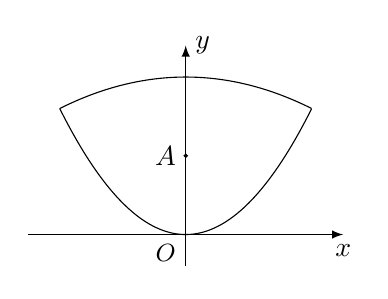
\begin{tikzpicture}[scale=0.4]
\coordinate[label=below left:\small$O$](O) at(0,0);
\coordinate[label=left:$A$](A) at (0,2.5);
\draw[fill] (A) circle (1.4pt); 
\draw[->,>=latex](-5,0)--(5,0)node[below](x){$x$};
\draw[->,>=latex](0,-1)--(0,6)node[right](x){$y$};
\draw[domain=-4:4,samples=1000] plot(\x,{1/4*(\x)^2});
\draw[domain=-4:4,samples=1000] plot(\x,{-1/16*(\x)^2+5});
\end{tikzpicture}
\end{center}
\onech{$ \left(1,3\right)$}{$ \left(2,4\right)$}{$ \left(\dfrac{3}{2},3\right)$}{$ \left(\dfrac{5}{2},4\right)$}
\qs 已知$ a,b $是正数,且满足$ 2<a+2b<4, ~$那么$ \dfrac{b+1}{a+1} $的取值范围是\xx
\twoch{$ \left(\dfrac{1}{5},3\right)$}{$ \left(\dfrac{1}{3},2\right)$}{$\left(\dfrac{1}{5},2\right) $}{$\left(\dfrac{1}{3},3\right) $}
\qs 设关于$ x,y $的不等式组$ \begin{dcases}
2x-y+1>0\\x+m<0\\y-m>0
\end{dcases} $
表示的平面区域内存在点$ P(x_0,y_0) $满足$ x_0-2y_0=2 $,求得$ m $的取值范围是\xx
\onech{$\left(-\infty,-\dfrac{4}{3}\right)$}{$\left(-\infty,-\dfrac{1}{3}\right)$}{$\left(-\infty,-\dfrac{2}{3}\right)$}{$\left(-\infty,-\dfrac{5}{3}\right)$}
\qs 已知$ \bm{e}_1 ,\bm{e}_2$为平面上的单位向量,$ \bm{e}_1 $和$ \bm{e}_2 $的起点均为坐标原点$ O $,~  $\bm{e}_1$与$\bm{e}_2$夹角为$ \dfrac{\pi}{3} .$平面区域$ D $由所有满足$ \vv{OP}=\lambda \bm{e}_1+\mu \bm{e}_1 $的点$ P $组成,其中$ \begin{dcases}
\lambda+\mu\le1,\\
0\le\lambda,\\
0\le\mu.
\end{dcases} $那么平面区域$ D $的面积为\xx
\onech{$ \dfrac{1}{2}$}{$ \sqrt{3}$}{$ \dfrac{\sqrt{3}}{2}$}{$ \dfrac{\sqrt{3}}{4}$}
\qs 已知符号函数$ sgn(x)=\begin{dcases}
1,&x>0,\\
0,&x=0,\\
-1,&x<0.
\end{dcases} $,则函数$f(x)=sgn(\ln x)-\ln^2x$的零点个数为\xx
\onech{$ 1$}{$ 2$}{$ 3$}{$ 4$}
\qs 设不等式组$ \begin{dcases}
x+y-11\ge 0\\3x-y+3\ge 0\\5x-3y+9\ge 0
\end{dcases} $表示的平面区域为$ D $,若指数函数$ y=a^x $的图象上存在区域$ D $上的点,则$ a $的取值范围是\xx
\onech{$\left(1,3\right]$}{$\left[2,3\right]$}{$\left(1,2\right]$}{$\left[3,+\infty\right)$}
\qs 如图,正方体$ ABCD-A_1B_1C_1D_1 $的棱长为$2$,动点$ E,F $在棱$ A_1B_1 $上,动点$ P,~Q $分别在棱$ AD,~CD $上,若$ EF=1,~A_1E=x,~DQ=y,~DP=z~(x,y,z\text{大于零} )$,则四面体$P-EFQ  $的体积
\xx
\fourch{与$ x,y,z $都有关}{与$ x $有关,与$ y,z $无关}{与$ y $有关,与$ x,z $无关}{与$ z $有关,与$ x,y $无关}
\vspace{-9em}
\\\mbox{\hspace{1pt}}\hfill
\begin{tikzpicture}
\draw (0,0) node[below](A) {\small$A$}--(2,0) node[below](B){\small$B$}--(2,2) node[right](B1){\small$B_1$}--(0,2) node[left](A1) {\small$A_1$}--(0,0)--cycle;
\draw[dashed] (0,0)--(0.76,0.76) node[left](D){\small$D$}--(2.76,0.76) node[right](C){\small$C$};
\draw (2.76,0.76)--(2,0);
\draw (0,2) --(0.76,2.76)node[left](D1){\small$D_1$}--(2.76,2.76)node[right](C1){\small$C_1$}--(2,2);
\draw [dashed](0.76,2.76)--(0.76,0.76) ;
\draw (2.76,2.76)--(2.76,0.76);
%\draw [dashed](0.76,2.76)--(2.38,0.38) node[right](E) {\small$E$};
\coordinate [label=\small$E$](E) at($(A1)!0.33!(B1)$) ;
\coordinate [label=\small$F$](F) at($(A1)!0.7!(B1)$) ;
\coordinate [label=\small$P$](P) at($(0,0)!0.33!(0.76,0.76)$) ;
\coordinate [label=\small$Q$](Q) at($(D)!0.5!(C)$) ;
%\draw[fill] (E) circle (1.1pt);
%\draw[fill] (F) circle (1.1pt);
%\draw[fill] (P) circle (1.1pt);
%\draw[fill] (Q) circle (1.1pt);
\foreach \p in{E,F,P,Q}
\draw[fill](\p) circle(1.1pt);
\end{tikzpicture}
\qs 如图,将一张边长为$ 1 $的正方形纸$ ABCD $折叠,使得点$ B $始终落在边$ AD $上,则折起部分面积的最小值为\xx
\onech{$ \dfrac{1}{4}$}{$ \dfrac{3}{8}$}{$ \dfrac{2}{5}$}{$ \dfrac{1}{2}$}
\begin{center}
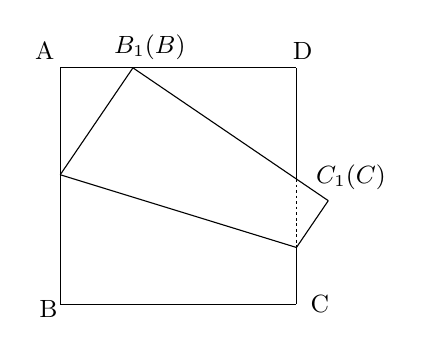
\begin{tikzpicture}[x=3cm,y=3cm]
%\clip(-0.1,-0.1) rectangle (1.3,1.2);
\draw (0.,1.)-- (1.,1.);
\draw (0.3078342226255113,1.)-- (0.,0.5473809543097264);
\draw (0.,0.5473809543097264)-- (1.,0.23954673168421506);
\draw (0.3078342226255113,1.)-- (1.1347154689068106,0.4376234317218708);
\draw (1.1347154689068106,0.4376234317218708)-- (1.,0.23954673168421506);
\draw [dash pattern=on 1pt off 1pt] (1.,0.5292458060815594)-- (1.,0.23954673168421506);
\draw (1.,1.)-- (1.,0.5292458060815594);
\draw (1.,0.23954673168421506)-- (1.,0.);
\draw (1.,0.)-- (0.,0.);
\draw (0.,1.)-- (0.,0.);
\begin{scriptsize}
%\draw [fill=black] (0.,0.) circle (2.5pt);
\draw[color=black] (-0.05,-0.02) node {\small B};
%\draw [fill=black] (1.,0.) circle (2.5pt);
\draw[color=black] (1.0262830428718939,0.) node[right] {\small C};
%\draw [fill=uuuuuu] (1.,1.) circle (2.5pt);
\draw[color=black] (1.0262830428718939,1.0714316919701667) node {\small D};
%\draw [fill=uuuuuu] (0.,1.) circle (2.5pt);
\draw[color=black] (-0.06604235459999686,1.0714316919701667) node {\small A};
%\draw [fill=black] (0.3078342226255113,1.) circle (2.5pt);
\draw[color=black] (0.37919897589126295,1.) node[above] {\small $B_1(B)$};
%\draw [fill=black] (1.1347154689068106,0.4376234317218708) circle (2.5pt);
\draw[color=black] (1.05,0.5351632450229179) node[right] {\small $C_1(C)$};
\end{scriptsize}
\end{tikzpicture}
\end{center}
\qs 一个几何体的三视图如图所示,那么该几何体的最长棱长为\xx
\begin{center}
\begin{tikzpicture}
\draw (0,0)--(2,0)--++(0,2)--cycle;
\node(P) at(1,-0.2){\tiny$2$};
\draw[->|,>=latex](P)--(0,-0.2);
\draw[->|,>=latex](P)--(2,-0.2);
\node (Q)at(2.2,1){\tiny$2$};
\draw[->|,>=latex](Q)--(2.2,2);
\draw[->|,>=latex](Q)--(2.2,0);
\node (r) at(1,-0.5){正视图};
\begin{scope}[xshift=3cm]
\draw (0,0)--+(2,0)--+(0,2)--cycle;
\draw (0,2)--(1,0);
\node(P) at(0.5,-0.2){\tiny$1$};
\draw[->|,>=latex](P)--(0,-0.2);
\draw[->|,>=latex](P)--(1,-0.2);
\node(P) at(1.5,-0.2){\tiny$1$};
\draw[->|,>=latex](P)--(1,-0.2);
\draw[->|,>=latex](P)--(2,-0.2);
\node (r) at(1,-0.5){侧视图};
\end{scope}
\begin{scope}[xshift=5.5cm,yshift=2cm]
\draw(0,0)--++(2,0)--++(0,-2)--++(-2,1)--cycle;
\draw (0,-1)--(2,0);
\node (r) at(1,-2.5){俯视图};
\end{scope}
\end{tikzpicture}
\end{center}
\vspace{-1em}
\onech{$ 2$}{$ 2\sqrt{2}$}{$ 3$}{$ \sqrt{10}$}
\qs 在平面直角坐标系$xOy$中,正四面体$ P-ABC $的顶点$ A,~B $分别在$x$轴,$y$轴上移动,若该正四面体的棱长为$ 2 $,则$ \abs{OP} $的取值范围是\xx
\twoch{$ \left[\sqrt{3}-1,\sqrt{3}+1\right]$}{$ \left[1,3\right]$}{$ \left[\sqrt{3}-1,2\right]$}{$ \left[1,\sqrt{3}+1\right]$}
\qs 某四棱锥的三视图如图所示,则该四棱锥的底面的面积是\xx
\begin{center}
\begin{tikzpicture}
\coordinate (p) at (0,0) {};
%\draw (p)--++(1,0)--++(0,1)--++(-1,0)--cycle;
\draw (p) rectangle +(2,2);
\draw[densely dashed,thin] (p)--($(p)+(2,2)$);
\draw ($(p)+(0,1)$)--($(p)+(2,0)$);
\node (p1) at (-0.2,1.5) {\tiny 0.5};
\draw[->|,>=stealth](p1)--($(p1)+(0,0.5)$);
\draw[->|,>=stealth](p1)--($(p1)+(0,-0.5)$);
\node (p2) at (1,2.2){\tiny 1};
\draw[->|,>=stealth](p2)--($(p2)+(1,0)$);
\draw[->|,>=stealth](p2)--($(p2)+(-1,0)$);
\node (s) at(1,-0.3){\small 正视图}; 
\begin{scope}[xshift=2.5 cm]
\coordinate (p) at (0,0);
\draw (p)--+(2,0)--+(2,2)--cycle;
\draw (p)--(2,1);
\node(p2) at (2.2,0.5){\tiny 0.5};
\draw [->|,>=stealth](p2)--($(p2)+(0,0.5)$);
\draw [->|,>=stealth](p2)--($(p2)+(0,-0.5)$);
\node (s) at(1,-0.3){\small 侧视图}; 
\end{scope}
\begin{scope}[yshift=-3cm]
\draw (0,0)--+(2,0)--+(0,2)--cycle;
\node (p) at(-0.2,1){\tiny 1};
\draw [->|,>=stealth](p)--(-0.2,2);
\draw [->|,>=stealth](p)--(-0.2,0);
\node (s) at(1,-0.3){\small 俯视图}; 
\end{scope}
\end{tikzpicture}
\end{center}
\onech{$ \dfrac{1}{2}$}{$ \dfrac{3}{2}$}{$ \dfrac{1}{4}$}{$ \dfrac{3}{4}$}
\qs 
如图,在等腰梯形$ ABCD $中,$ AB=8,~BC=4,~CD=4,~ $点$ P $在线段$ AD $上运动,则$\left|\vv{PA}+\vv{PB}\right| $的取值范围是\xx
\onech{$ \left[6,4+4\sqrt{3}\right] $}{$\left[4\sqrt{2},8\right] $}{$ \left[4\sqrt{3},8\right] $}{$ \left[6,12\right] $}
\vspace{-2em}
\begin{center}
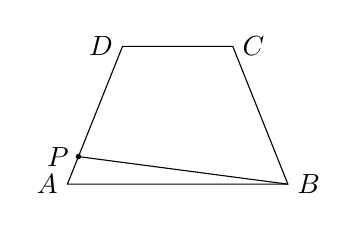
\begin{tikzpicture}[scale=0.7]
%\draw[help lines] (0,0) grid (4,4);
\draw (0,0) node[left](A){$A$} --(4,0)node[right](B){$B$} -- (3,2.5) node[right](C) {$C$}--(1,2.5) node[left](D){$D$}--cycle;
\coordinate[label=left:$P$] (P) at (0.2,0.5);
\draw[fill] (P) circle (1.1pt); 
\draw (P)--(4,0);
\end{tikzpicture}
\end{center}
\qs 在三角形$\triangle ABC$中,点$ D $满足$ \vv{AD}=2\vv{AB}-\vv{AC} $,则\xx
\twoch{点$ D $不在直线$ BC $上}{点$ D $在$ BC $的延长线上}{点$ D $在线段$ BC $上}{点$ D $在$ CB $的延长线上}
\qs $\vv{a},\vv{b} $为非零向量,“$ \vv{a}\bot\vv{b} $”是“函数$ f(x)=(x\vv{a}+\vv{b})\bm\cdot(x\vv{b}-\vv{a}) $为一次函数”的\xx
\twoch{充分而不必要条件}{必要而不充分条件}{充分必要条件}{既不充分也不必要条件}
\qs 现有10支队伍比赛,规定:比赛采取单循环比赛制,每支队伍与其他9支队伍各比赛一场,每场比赛中,胜方得2分,负方得0分,平局双方各得1分.下面关于这10支队伍得分的叙述正确的是\xx
\twoch{可能有两支队伍得分都是18分}{各队得分总和为180分}{各支队伍中最高得分不少于10分}{得偶数分的队伍必有偶数个} 
\qs 袋中装有偶数个球,其中红球、黑球各占一半,甲、乙、丙是三个空盒,每次从袋中任意取出两个球,将其中一个放入甲盒,如果这个球是红球,就将另一个球放入乙盒,如果这个球是黑球,就将另一个球放入丙盒,重复上述过程,直到袋中所有球都被放入到盒中,则\xx
\fourch{乙盒中黑球不多于丙盒中黑球}{乙盒中红球与丙盒中黑球一样多}{乙盒中红球不多于丙盒中红球}{乙盒中黑球和丙盒中红球一样多}
\qs 有语文,数学两门学科,成绩评定为“优秀”,“合格”,“不合格”三种,若$A$同学每科成绩不低于$B$同学,且至少有一科成绩比$B$高,则称“$A$同学比$ B $同学成绩好.”现有若干同学,他们之间没有一个人比另一个成绩好,且没有任意两个人的语文成绩一样,数学成绩也一样的,问满足条件的最多有多少学生\xx
\onech{2}{3}{4}{5}
\qs 为提高信息在传输中的抗干扰能力,通常在原信息中按照一定规则加入相关数据组成传输信息,设定原信息为$ a_0a_1a_2 $,其中$ a_i\in\left\{0,1\right\}(i=0,1,2) $,传输信息为$ h_0a_0a_1a_2h_1,~h_0=a_0\oplus a_1,~h_1=h_0\oplus a_2 $,$ \oplus $运算规则为:$ 0\oplus 0=0,~0\oplus 1=1,~1\oplus 0=1,~1\oplus 1=0. $例如原信息为$ 111 $,则传输信息为$ 01111.~ $传输信息在传输过程中受到干扰可能导致接收信息出错,则下来信息一定错误的是\xx
\onech{$ 11010$}{$ 01100$}{$ 10111$}{$ 00011$}
\end{questions}






\newpage
\section{填空}
\begin{questions}
\qs 已知函数$f(x)=\Bigg\{\begin{aligned}
&\dfrac{2}{x},&x\ge2\\
&(x-1)^3,&x<2.
\end{aligned}$若关于$ x $的方程$ f(x)=k $有两个不同的实根,则数$ k $的取值范围是\tk.

\qs
设函数$f(x)=\Bigg\{\begin{aligned}
&~2^x-a,& x<1;\\
&~4(x-a)(x-2a),& x\ge 1.
\end{aligned}$\\
\ding{192}~若$a=1$,则$ f(x) $的最小值为\tk;\\
\ding{193}~若$f(x) $恰有$ 2 $个零点,则实数$ a $的取值范围是\tk.
\qs 设函数$f(x)=\begin{dcases}
x^3-3x,&x\le a \\
-2x,&x>a.
\end{dcases}$\\
\ding{192} 若$ a=0 $,则$f(x)$的最大值为\tk;\\
\ding{193} 若$f(x)$无最大值,则实数$ a $的取值范围是\tk.
\qs 关于$ x $的方程$ g(x)=t(t\inR) $的实数根的个数记为$ f(t) $,若$g(x)=\ln x$,则$f(t)=$\tk;若$g(x)=\Bigg\{\begin{aligned}
&x,&x\le0;\\
&-x^2+2ax+a,&x>0.
\end{aligned}(a\inR)$,存在$ t $使得$ f(t+2)>f(t) $成立,则$ a $的取值范围是\tk.
\qs 已知函数$f(x)=\Bigg\{\begin{aligned}
&(x-2a)(a-x),&x\le 1,\\&\sqrt{x}+a-1,&x>1.
\end{aligned}$
\begin{parts}
\part 若$ a=0,~x\in\left[0,4\right],~ $则$f(x)$的值域为\tk;
\part 若$f(x)$恰有三个零点,则实数$ a $的取值范围是\tk.
\end{parts}
\qs 已知函数$f(x)=\Bigg\{\begin{aligned}
&1-x^2,&x\ge 0,\\
&\cos \pi x,&x<0.
\end{aligned}$若关于$ x $的方程$ f(x+a)=0 $在$ (0,+\infty) $内有唯一实根,则实数$ a $的最小值是\tk.
\qs 设$ f(x)=\Bigg\{\begin{aligned}
&x^3,&x<a,\\
&x^2,&x\ge a.
\end{aligned} $若存在实数$ b $,使得函数$ g(x)=f(x)-b $有两个零点,则$ a $的取值范围是\tk.
\qs 已知函数$f(x)$是$\mathbf{R}$上的减函数,且$y=f(x-2)$的图象关于点$ (2,0) $成中心对称,若$ u,v $满足不等式组$\Bigg\{\begin{aligned}
&f(u)+f(v-1)\le 0,\\
&f(u-v-1)\ge 0.
\end{aligned}$则$ u^2+v^2 $的最小值是\tk.
\qs 已知函数$f(x)=m(x-2m)(x+m+3),g(x)=2^x-2$,若$ \forall x\inR ,f(x)<0$或$ g(x)<0,~ $则$ m $的取值范围是\tk.
\qs 已知定义在$ \left(0,+\infty\right) $的函数$f(x)$的导函数$f'(x)$是连续不断的,若方程$f'(x)=0$无解,且$ \forall x\in\left(0,+\infty\right) ,~f\left[f(x)-\log_{2016}x\right]=2017,~$设$ a=f\left(2^{0.5}\right),~b=f\left(\log_43\right),~c=f\left(\log_{\pi}3\right),~ $则$ a,~b,~c $的大小关系是\tk.
\question
若函数$f(x)=(1-x^2)(x^2+ax+b)$的图象关于直线$x=-2$对称,则$f(x)$的最大值是\tk.
\qs 已知函数$f(x)=e^x-e^{-x}(x\inR,\text{且}e\text{为自然对数的底}).$若存在实数$ t,~ $使不等式$ f(x-t)+f(x^2-t^2)\ge 0 $对一切的$ x\inR $都成立,则$ t= $\tk.

\qs 已知函数$f(x)=\cos x-2^x-2^{-x}-b,~(b \inR)$.
\begin{parts}
\part 当$ b=0 $时,函数$f(x)$的零点个数为\tk; 
\part 若函数$f(x)$有两个不同的零点,则$ b $的取值范围是\tk.
\end{parts}
\qs 已知函数$f(x)$为偶函数,且$ x\ge 0 $,$f(x)=x-\left[x\right](\left[x\right]\text{表示不超过}x\text{的最大整数})$.设$g(x)=f(x)-kx-k(k\inR)$,若$ k=1 $,则函数$g(x)$有\tk 个零点;若$g(x)$有三个不同零点,则$ k $的取值范围是\tk.
\qs 已知函数$f(x)=m(x-2m)(x+m+3),~g(x)=2^x-2.$若同时满足条件:\\
\ding{192} $ \forall x \in \mathbf{R} ,~f(x)<0~\text{或}~g(x)<0;$\\
\ding{193} $ \exists x \in (-\infty,-4),~f(x)g(x)<0, $\\
则$ m $的取值范围是\tk.

\qs 已知函数$f(x)=\abs{\ln x }$,关于$ x $的不等式$ f(x)-f(x_0)\ge c(x-x_0) $的解集为$ \left(0,+\infty\right),~ $其中$ x_0\in \left(0,+\infty\right),c\text{为常数} .$当$ x_0=1 $时,$ c $的取值范围是\tk;当$ x_0=\dfrac{1}{2} $时,$ c $的值是\tk.

\qs 已知函数$f(x)=\lg\left[mx^2+(m+2)x+2(m+2)\right]$.
\begin{parts}
\part 若函数$f(x)$的定义域为$\mathbf{R}$,则实数$ m $的取值范围是\tk;
\part 若函数$f(x)$在区间$ \left[m+2,2(m+2)\right] $上恒有定义,则实数$ m $的取值范围是\tk.
\end{parts}
\qs 已知函数$f(x)$,对于实数$ t $,若存在$ a>0,~b>0$,满足$ \forall x\in [t-a,t+b] $,使得$ \left|f(x)-f(t)\right|\le 2,~ $则记$ a+b $的最大值为$ H(t) .$
\begin{parts}
\part 当$ f(x)=2x $时,$ H(0)= $\tk;
\part 当$ f(x)=x^2 $且$ t\in[1,2] $时,函数$ H(t) $的值域为\tk.
\end{parts}


\qs 曲线$C$是平面内与两个定点$ F_1(-1,0) $和$F_2(1,0)$的距离的积等于常数$ a^2 $的点的轨迹.给出下列三个结论:\\
\ding{192} 曲线$ C $过坐标原点;\\
\ding{193} 曲线$ C $关于坐标原点对称;\\
\ding{194} 若点$ P $在曲线$ C $上,则$ \triangle F_1PF_2 $的面积不大于$ \dfrac{1}{2}a^2. $\\
其中,所有正确的结论的序号是\tk.
\qs 若点$O$和点$F_2(-\sqrt{2},0) $分别为$\dfrac{x^2}{a^2}-y^2=1~(a>0)$的中心和左焦点,点$ P $为双曲线右支上的任意一点,则$ \dfrac{\abs{PF_2}^2}{\abs{OP}^2+1} $的取值范围为\tk.
\qs 已知函数$ f(x)=e^x-e^{-x} ,~$下列命题正确的有\tk.(写出所有正确命题的编号)\\
\ding{192}$f(x)$是奇函数;\\
\ding{193}$f(x)$在$ \mathbf{R} $上是单调递增函数;\\
\ding{194}方程$ f(x)=x^2+2x $有且仅有$ 1 $个实数根;\\
\ding{195}如果对于任意$ x\in (0,+\infty),~ $都有$ f(x)>kx,~ $那么$ k $的最大值为2.
\qs 如图放置的边长为$1$的正方形$PABC$沿$x$轴滚动.设顶点
$P(x,y)$的轨迹方程是$ y=f(x) $,则$f(x)$的最小正周期为\tk;$y=f(x)$在其两个相邻零点间的图像与$x$轴所围区域的面积为\tk.\par
\vspace{-1em}
\begin{center}
\begin{tikzpicture}
\tikzmath{
\a=sin(45);
\b =\a;
\c=2*\a;
}
\draw[->,>=latex] (-1,0)--(2,0) node[below](x){$x$};
\draw[->,>=latex] (0,-1)--(0,2) node[left](y){$y$};
\coordinate [label=below left:$O$](O) at (0,0);
\draw  (\a,0) node[below](A){\small$A$}--(\c,\a)node[right](B){\small$B$}--(\a,\c)node[above](C){\small$C$}--(0,\a)node[left](P){\small$P$}--cycle;
\end{tikzpicture}
\end{center}
\vspace{-1em}
{\kaishu {\heiti 说明:}“正方形$PABC$沿$x$轴滚动”包括沿$x$轴正方向和沿$x$轴负方向滚动.沿$x$轴正方向滚动指的是先以顶点$A$为中心顺时针旋转,当顶点$B$落在$x$轴上时,再以顶点$B$为中心顺时针旋转,如此继续.类似地,正方形$PABC$可以沿$x$轴负方向滚动.}

\qs 在平面直角坐标系$xOy$中,动点$ P(x,y) $到两坐标轴的距离之和等于它到定点$ (1,1) $的距离,记点$ P $的轨迹为$ C $,给出下面四个结论:\\
\ding{192} 曲线$ C $关于原点对称;\\
\ding{193} 曲线$ C $关于$ y=x $对称;\\
\ding{194} 点$ (-a^2,1)(a\inR) $在曲线$ C $上;\\
\ding{195} 在第一象限,曲线$ C $与$x$轴的非负半轴、$y$轴的非负半轴围成的封闭图形的面积小于$ \dfrac{1}{2}. $\\
其中所有的正确结论的序号是\tk.
\qs 如图,在直角梯形$ ABCD $中,$ AB\sslash CD,~AB\bot BC,~AB=2,~CD=1,~BC=a~(a>0),~ P$为线段$ AD $上一个动点,设$ \vv{AP}=x\vv{AD},~ \vv{PB}\bm{\cdot}\vv{PC}=y,~$对于函数$y=f(x),~$给出以下三个结论:\\
\ding{192} 当$ a=2 $时,函数$f(x)$的值域为$ \left[1,4\right] $;\\
\ding{193} $ \forall a\in\left(0,+\infty\right),~$都有$ f(1)=1 $成立;\\
\ding{194} $ \forall a\in\left(0,+\infty\right),~$函数$f(x)$的最大值都等于$ 4 $.\\
其中所有正确结论的序号是\tk.
\vspace{-7em}
\begin{flushright}
\begin{tikzpicture}[scale=1.2]
%\draw[help lines](0,0) grid (2.2,2.2);
\coordinate[label=below:$A$](A) at(0,0);
\coordinate[label=below:$B$](B) at(2,0);
\coordinate[label=left:$D$](D) at(1,2);
\coordinate[label=right:$C$](C) at(2,2);
\coordinate[label=left:$P$] (P) at($(A)!0.5!(D)$);
\draw (A)--(B)--(C)--(D)--cycle (B)--(P)--(C);
%\node(bq) at(2.1,0){$\text{图}1$};
\end{tikzpicture}
\end{flushright}
\qs 如图,$ \triangle AB_1C_1,~\triangle C_1B_2C_2,~\triangle C_2B_3C_3 $是三个边长为2的等边三角形,且有一条边在同一直线上,边$ B_3C_3 $上有两个不同的点$ P_1,~P_2,~ $则$ \vv{AB_2}\bm{\cdot}(\vv{AP_1}+\vv{AP_2}) =$\tk.

\begin{center}
\begin{tikzpicture}
\tikzmath{
\a=sqrt(3);
}
\coordinate[label=below:$A$](A) at (0,0);
\foreach \p in {1,2,3}
\coordinate[label=below:$C_{\p}$] (C_\p) at($(\p*2,0)$) ;
\foreach \q in {1,2,3}
\coordinate[label=above:$B_{\q}$] (B_\q) at($(2*\q-1,\a)$);
\foreach \r in{1,2,3}
\draw (B_\r)--(C_\r);
\draw (A)--(C_3) (A)--(B_1) (C_1)--(B_2) (C_2)--(B_3);
\draw[->,>=stealth] (A)--(B_2) ;
\draw[->,>=stealth](A)--($(B_3)!0.3!(C_3)$) node[right](P_1){$P_1$};
\draw[->,>=stealth](A)--($(B_3)!0.7!(C_3)$) node[right](P_2){$P_2$};
\end{tikzpicture}
\end{center}
\qs 已知函数$f_n(x)=\dfrac{\sin nx}{\sin x}~(n\in\mathbf{N^*})$,关于此函数的说法正确的序号是\tk\par
\begin{tabular}{ll}
\ding{192} $ f_n(x)(n\in\mathbf{N^*}) $为周期函数;&\ding{193} $f_n(x)(n\in\mathbf{N^*})$有对称轴; \\
\ding{194} $ \left(\dfrac{\pi}{2},0\right) $为$ f_n(x)(n\in\mathbf{N^*}) $的对称中心;&\ding{195} $ \abs{f_n(x)}\le n(n\in\mathbf{N^*})$.
\end{tabular}
\qs 向量$ \vv{a},\vv{b},\vv{c} $在正方形网格中的位置如图所示,若$ \vv{c}=\lambda\vv{a}+\mu\vv{b}~(\lambda,\mu \in \mathbf{R}) $,则$ \dfrac{\lambda}{\mu}=$\tk.
\begin{center}
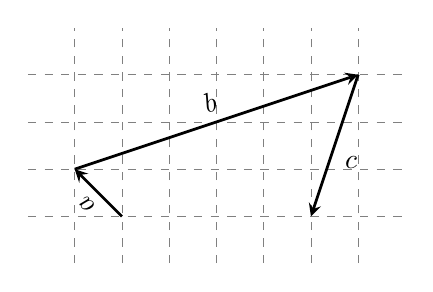
\begin{tikzpicture}[line width=1 pt,scale=0.6]
\draw[help lines,smooth, dashed] (-3.99,-2.99) grid (3.99,1.99);
\draw [->,>=stealth](-2,-2)--(-3,-1) node[sloped,midway,left,above,rotate=180](a){$\large\vv{a}$};
\draw [->,>=stealth](-3,-1)--(3,1) node[sloped,midway,left,above](b){$\large\vv{b}$};
\draw [->,>=stealth](3,1)--(2,-2) node[midway,below right ](c){$\large\vv{c}$};
\end{tikzpicture}
\end{center}
\qs 如图,在平行四边形$ ABCD $中,$ AP\bot BD~ $,垂足为$ P $,且$ AP=3 $,则$\vv{AP}\bm{\cdot}\vv{AC}= $\tk.\begin{center}
\begin{tikzpicture}
%\draw[help lines](0,0) grid (4,4);
\coordinate [label=below:$B$](B) at(0,0);
\coordinate [label=below:$C$](C) at(3,0);
\coordinate [label=$A$](A) at(1,1.5);
\coordinate [label=$D$](D) at(4,1.5);
\draw (A)--(B)--(C)--(D)--cycle (A)--(C) (B)--(D);
\coordinate[label=below:$P$] (P) at($(B)!(A)!(D)$);
\draw (A)--(P);
\end{tikzpicture}
\end{center}

\qs 给定两个长度为$ 1 $的平面向量$ \vv{OA} $和$ \vv{OB} $,它们的夹角为$ 120^{\circ} $.如图所示,点$ C $在以$ O $为圆心的圆弧$ \wideparen{AB} $上变动,若$ \vv{OC}=x\vv{OA}+y\vv{OB} $,其中$ x,~y\inR $,则$ x+y $的最大值是\tk.
\begin{center}
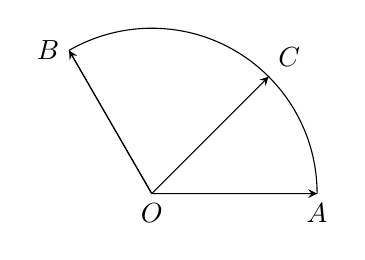
\begin{tikzpicture}[scale=0.7]
\coordinate[label=below:$O$](O) at(0,0);
\coordinate[label=below:$A$](A) at(0:3);
\coordinate[label=left:$B$](B) at(120:3);
\draw (O)--(A) (O)--(B);
\draw (3,0) arc (0:120:3);
\coordinate [label=above right:$C$](C) at(45:3);
\foreach \p in {A,B,C}
\draw[->,>=stealth](O)--(\p);
\end{tikzpicture}
\end{center}
\qs 如图,在棱长为$2$的正方体$ ABCD-A_1B_1C_1D_1 $中,$ E $为$ BC $中点,点$ P $在线段$ D_1E $上,点$ P $到直线$ CC_1 $的距离的最小值为\tk.
\begin{center}
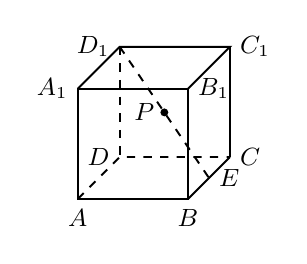
\begin{tikzpicture}[line width=0.7 pt,scale=0.7]
%\draw[help lines] (0,0) grid (3,3);
\draw (0,0) node[below](A) {\small$A$}--(2,0) node[below](B){\small$B$}--(2,2) node[right](B1){\small$B_1$}--(0,2) node[left](A1) {\small$A_1$}--(0,0)--cycle;
\draw[dashed] (0,0)--(0.76,0.76) node[left](D){\small$D$}--(2.76,0.76) node[right](C){\small$C$};
\draw (2.76,0.76)--(2,0);
\draw (0,2) --(0.76,2.76)node[left](D1){\small$D_1$}--(2.76,2.76)node[right](C1){\small$C_1$}--(2,2);
\draw [dashed](0.76,2.76)--(0.76,0.76) ;
\draw (2.76,2.76)--(2.76,0.76);
\draw [dashed](0.76,2.76)--(2.38,0.38) node[right](E) {\small$E$};
\coordinate[label=left:\small$P$] (P) at (1.57,1.57);
\draw[fill] (P) circle (1.5pt) ;
\end{tikzpicture}
\end{center}

 




 \qs
设函数$ f(x)=A\sin (\omega x+\varphi)~(A,\omega,\varphi \text{是常数,}A>0,\omega>0)$.若$ f(x) $在区间$ \left[\dfrac{\pi}{6},\dfrac{\pi}{2}\right] $上具有单调性,且$f(\dfrac{\pi}{2})=f(\dfrac{2\pi}{3})=-f(\dfrac{\pi}{6}) $,则$ f(x) $的最小正周期是\tk.


\qs 实数$ a,~b $满足$ 0<a\le 2,~b\ge 1 $,若$ b\le a^2 $,则$ \dfrac{b}{a} $的取值范围是\tk.



\qs 已知实数$ u,v,x,y $满足$ u^2+v^2=1,~\begin{dcases}
x+y-1\ge 0,\\
x-2y+2\ge 0,\\
x\le 2.
\end{dcases} $则$ z=ux+vy $的最大值是\tk.
\qs 已知函数$f(x)=\begin{dcases}
1,&0\le x\le \dfrac{1}{2},\\
-1,&\dfrac{1}{2}\le x<1,\\
0,&x<0\text{或}x\ge 1
\end{dcases}$和$ g(x)=\Bigg\{\begin{aligned}
&1,\quad 0\le x<1,\\
&0,\quad x<0\text{或}x\ge1.
\end{aligned} $则:\\
$(\mathrm{1})$~$ g(2x)= $\tk ;\\
$(\mathrm{2})$若$ m,~n\inZ $且$m\bm\cdot g(n\bm \cdot x)-g(x)=f(x)$,则$ m+n= $\tk.

\qs 为了促销某电子产品,商场进行降价,设$ m>0,~n>0,~m\ne n,~ $有三种降价方案:\\
方案\ding{192}: 先降$ m\%,~ $再降$n\%  $;\\
方案\ding{193}:先降$ \dfrac{m+n}{2}\% $,再降$ \dfrac{m+n}{2}\% $\\
方案\ding{194}:一次性降价$ \left(m+n\right) \%$.\\
则降价幅度最小的方案是\tk.(填出正确的序号)

\qs 如图,正方体$ABCD-A_1B_1C_1D_1$的棱长为$2$,点$ P $在正方形$ ABCD $的边界及其内部运动,平面区域$ W $由所有满足$ A_1P\le \sqrt{5} $的点$ P $组成,则$ W $的面积是\tk;四面体$ P-A_1BC $的体积的最大值是\tk.
\begin{center}
\begin{tikzpicture}
\tikzmath{
\a=cos(45);
\b =sin(45);
\c=1*\a ;
\d =1*\b ;
}
\coordinate[label=left:$A$](A) at (0,0);
\coordinate[label=right:$B$](B) at (2,0);
\coordinate[label=above right:$D$](D) at(\c,\d);
\coordinate[label={right,above}:$C$](C) at($(B)+(\c,\d)$);
\foreach \p in{B,C}
\coordinate[label=right:$\p_1$](\p_1) at($(\p)+(0,2)$);
\foreach \p in{A,D}
\coordinate[label=left:$\p_1$](\p_1) at($(\p)+(0,2)$);
\draw (A)--(B)--(C)--(D)--cycle;
\draw (A_1)--(B_1)--(C_1)--(D_1)--cycle;
\foreach \p in{A,B,C,D}
\draw (\p)--(\p_1);
\coordinate[label=above right:$P$](P) at(0.4,0.2);
\draw[dashed](P)--(B) (P)--(C) (P)--(A_1) (A_1)--(C);
\end{tikzpicture}
\end{center}


\qs 设关于$ x,y $的不等式组$ \Bigg\{\begin{aligned}
&3x-4\ge 0,\\
&\left(y-1\right)\left(3x+y-6\right)\le 0.
\end{aligned} $表示的区域为$ D. $已知点$ O(0,0),~A(1,0) $,点$ M $是$ D $上的动点,$ \vv{OA}\cdot\vv{OM}=\lambda \abs{\vv{OM}} $,则$ \lambda $的取值范围是\tk.

\qs 如图,定义坐标系$ xOy $,已知$ \bm{e}_1 $与$ \bm{e}_2 $分别与$x$轴和$y$轴正方向相同的单位向量,$\bm{e}_1$与$\bm{e}_2$夹角为$ \dfrac{\pi}{3} $,若$ \vv{OP}=x\bm{e}_1+y\bm{e}_2 $,则称$ (x,y) $是点$ P $的坐标.在此定义下,$ \angle xOy $平分线所在直线方程是\tk;以$ O $为圆心,$ 1 $为半径的圆的方程是\tk.
\begin{center}
\begin{tikzpicture}

\tikzmath{
\a =1.5*cos(60);
\b =1.5*sin(60);
}
\coordinate[label=below:$O$] (O) at(0,0);
\draw[->,>=latex] (-1,0)--(3,0) node[below] (x){$x$};
\draw[->,>=latex] (60:-1)--(60:3) node[right] (y){$y$};
\draw[dashed] (\a ,\b)--($(1.5,0)+(\a,\b)$)node[right] (P) {$P$}--(1.5,0);
\draw[fill] ($(1.5,0)+(\a,\b)$) circle (1pt);
\draw[->,>=stealth] (0,0)--(60:1) node[midway, sloped,above ](e2){$\bm{e}_2$} ;
\draw[->,>=stealth] (0,0)--(1,0) node[midway,below ](e1){$\bm{e}_1$};
\end{tikzpicture}
\end{center}

\qs 已知向量序列:$ \bm{a}_1,\bm{a}_2,\bm{a}_3,\cdots,\bm{a}_n,\cdots $满足如下条件:$ \left|\bm{a}_1\right|=4\left|\bm{d}\right|=2,~2\bm{a}_1\bm\cdot \bm{d}=-1 $且$ \bm{a}_n-\bm{a}_{n-1}=
\bm{d}~(n=,3,4,\cdots). $若$ \bm{a}_1\bm{\cdot}\bm{a}_k=0,~ $则$ k= $\tk;~$ \left|\bm{a}_1\right|,~  \left|\bm{a}_2\right|, \left|\bm{a}_3\right|,\cdots, \left|\bm{a}_n\right|,\cdots$中第\tk 项最小.
\qs 把$ 5 $件不同的产品摆成一排,若产品$ A $与产品$ B $相邻,且产品$ A $不与产品$ C $相邻,则不同的摆法有\tk 种.
\qs 10名象棋选手单循环赛(即没两名选手比赛一场),规定两人对局胜者得$ 2 $分, 平局各得$ 1 $分,负者得$ 0 $分,并按总得分由高到低进行排列.比赛结束后,$ 10 $名选手的得分各不相同,且第二名的成绩是最后五名选手得分之和的$ \dfrac{4}{5} $.则第二名选手的得分是\tk. 



\qs 已知甲,~乙,~丙三人组成考察小组,每个组员最多可以携带供本人在沙漠中生存36天的水和食物,且计划每天向沙漠深处走30公里,每个人都可以在沙漠中将部分水和食物交给其他人然后独自返回,若组员甲与其他两个人合作,且要求三个人都能够安全返回,则甲最远能深入沙漠\tk 公里.
\qs 在某中学的“校园微电影节”活动中,学校将从微电影的“点播量”和“专家评分”两个角度来进行评优. 若$A$电影的“点播量”和“专家评分”中至少有一项高于$B$电影,则称$A$电影不亚于$B$电影. 已知共有$10$部微电影参展,如果某部电影不亚于其他$9$部,就称此部电影为优秀影片. 那么在这$10$部微电影中,最多可能有\tk 部优秀影片.
\qs 某网店统计了连续三天售出商品的种类情况:第一天售出$ 19 $种商品,第二天售出$ 13 $种商品,第三天售出$ 18 $种商品,前两天都售出的商品有$ 3 $种,后两天都售出的商品有$ 4 $种.
\begin{parts}
\part 则该网店第一天售出但第二天未售出的商品有\tk 种;
\part 这三天售出的商品最少有\tk 种.
\end{parts}
\qs 某学习小组由学生和教师组成,人员构成同时满足以下三个条件:\\
\begin{enumerate}[(i)]
\item 男学生人数多于女学生人数;
\item 女学生人数多于教师人数;
\item 教师人数的两倍多于男学生人数.
\end{enumerate}
\ding{192} 若教师人数为$ 4 $,则女学生人数的最大值为\tk;\\
\ding{193} 该小组的人生的最小值是\tk.

\end{questions}
\newpage
\section{压轴}
\begin{questions}
\qs (2016)设数列$ A:a_1,a_2,\cdots,a_N~(N\ge2) $.如果对小于$ n~(2\le n\le N) $的每个正整数$ k $都有$ a_k<a_n $,则称$ n $是数列$ A $的一个“$ G $时刻”.记$ G(A) $是数列$ A $的所有“$ G $时刻”组成的集合.
\begin{parts}
\part 对数列$ A:-2,2,-1,1,3 $,写出$ G(A) $的所有元素;
\part 证明:若数列$ A $中存在$ a_n $使得$ a_n>a_1 $,则$ G(A)\ne \varnothing $;
\part 证明:若数列$ A $满足$ a_n-a_{n-1}\le 1~(n=2,3,4,\cdots,N) $,则$ G(A) $的元素个数不小于$ a_N-a_1 $.
\end{parts}

\newpage
\qs (2015)已知数列$\{a_n\}$满足$ a_1\in\mathbf{N^*} ,~a_1\le 36$,且$ a_{n+1}=\Bigg\{\begin{aligned}
&2a_n,&a_n\le18\\
&2a_{n}-36,&a_n>18
\end{aligned} ~(n=1,2,3\cdots)$,记集合$ M=\left\{a_n\left|n\in \mathbf{N^*}\right.\right\} .$
\begin{parts}
\part 若$ a_1=6,~ $写出集合$ M $的所有元素;
\part 若集合$ M $存在一个元素是$ 3 $的倍数,证明:$ M $的所欲元素都是$ 3 $的倍数;
\part 求集合$ M $的元素个数的最大值.
\end{parts} 
\newpage
\qs (2014)对于数对序列$ P:(a_1,b_1),~(a_2,b_2),~(a_3,b_3),~\cdots,(a_n,b_n) $,记$ T_1(P)=a_1+b_1 $,$ T_k(P)=b_k+max\left\{T_{k-1}(P),a_1+a_2+a_3+\cdots+a_k\right\}~(2\le k\le n) $.其中$max\left\{T_{k-1}(P),a_1+a_2+a_3+\cdots+a_k\right\}$表示$ T_{k-1}(P) $和$ a_1+a_2+\cdots a_k $两个数中最大的数.
\begin{parts}
\part 对于数对序列$ P:(2,5),(4,1) $,求$ T_1(P),~T_2(P) $的值;
\part 记$ m $为$ a,b,c,d $四个数中最小值,对于由两个数对$ (a,~b),~(c,~d) $组成的数对序列$ P(a,b),~(c,d) $和$ P'(c,d),~(a,b) $,试分别对$ m=a $和$ m=d $的两种情况比较$ T_2(P) $和$ T_2(P') $的大小;
\part 在由5个数对$ (11,8),~(5,2),~(16,11),~(11,11),~(4,6) $组成的所有数对序列中,写出一个数对序列$ P $使$ T_5(P) $最小,并写出$ T_5(P) $的值.(只需写出结论)
\end{parts}
\newpage
\qs (2013)已知$\{a_n\}$是由非负整数组成的无穷数列,该数列前$n$项的最大值记为$A_n$,第$n$项之后各项$ a_{n+1} ,~a_{n+2}\cdots$的最小值记为$B_n,~d_n=A_n-B_n$.
\begin{parts}
\part 若$ \left\{a_n\right\} $为$2,~1,~4,~3,~3,2,~1,~4,~3\dots  $是一个周期为$ 4 $的数列~(即对任意$ n\in \mathbf{N^*}  ,a_{n+4}=a_n$),写出$ d_1,~d_2,~d_3,~d_4 $的值;
\part 设$ d $为非负整数,证明:$ d_n=-d~(n=1,2,3\cdots) $的充分必要条件为$ \left\{a_n\right\} $为公差为$ d $的等差数列;
\part 证明:若$ a_1=2,d_n=1~(n=1,2,3\dots) $,若$ \left\{a_n\right\} $的项只能是$ 1 $或$ 2 $,且有无穷多项$ 1 $.
\end{parts}
\newpage
\qs (2012)设$A$是由$ m\times n $个实数组成的$m$行$n$列的数表,满足:每个数的绝对值不大于$1$,且所有数的和为零,记$ S(m,n) $为所有这样的数表构成的集合.\\
对于$ A\in S(m,n) $,记$ r_i(A) $为$ A $的第$ i $行各数之和$ (1\le i\le m) $,$ c_i(A) $为$ A $的第$ j $列各数之和$(1\le j\le n)$;记$ k(A) $为$ \abs{r_1(A)},\abs{r_2(A)},\cdots,\abs{r_m(A)},\abs{c_1(A)},\abs{c_2(A)},\cdots,\abs{c_n(A)} $中的最小值.
\begin{parts}
\part 对如下数表$ A $,求$ k(A) $的值:
\begin{center}
\begin{tabular}{|c|c|c|}
\hline
1 &1 & -0.8\\
\hline
0.1 &-0.3 &-1\\
\hline
\end{tabular}
\end{center}

\part 设数表$ A\in S(2,3) $形如
\begin{center}
\begin{tabular}{|c|c|c|}
\hline
1 &1 & c\\
\hline
a &b &-1\\
\hline
\end{tabular}
\end{center}
求$ k(A) $的最大值;
\part 给定正整数$t$,对于所有的$ A\in S(2,2t+1) $,求$k(A)$的最大值.
\end{parts}
\newpage
\qs (2011)若数列$ A_n=a_1,a_2,\cdots,a_n~(n\ge 2) $满足$ \left|a_{k+1}-a_k\right|=1~(k=1,2,\cdots,n-1) $,数列$ A_n $为$ E $数列,记$ S(A_n)=a_1+a_2+a_3+\cdots+a_n.$
\begin{parts}
\part 写出一个满足$ a_1=a_5 =0$且$ S(A_5)>0 $的$ E $数列$ A_n $;
\part 若$ a_1=12,~n=2000 $,证明:$E$数列$ A_n $是递增数列的充要条件是$ a_n=2011 $;
\part 对任意给定的整数$n(n\ge 2) $,是否存在首项为$ 0 $的$ E $数列$ A_n $,使得$ S(A_n)=0 $?如果存在,写出一个满足条件的$ E $数列$ A_n $;如果不存在,说明理由.
\end{parts}
\kongbai
\qs (2010)已知集合$ S_n=\left\{X\left|X=(x_1,x_2,\cdots,x_n),~x_1\in \left\{0,1\right\},i=1,2,\cdots,n \right.\right\}~(n\ge 2) $,对于$ A=(a_1,a_2,\cdots,a_n) ,B=(b_1,b_2,\cdots,b_n)\in S_n$,定义$ A $与$ B $的差为$ A-B=\left(\abs{a_1-b_1},~\abs{a_2-b_2},\cdots,\abs{a_n-b_n}\right)$;\linebreak[2]$ A$与$ B $之间的距离为$ d(A,B)=\sum\limits_{i=1}^{n}\abs{a_i-b_i} $.
\begin{parts}
\part 证明:$ \forall A,~B,~C\in S_n $,有$ A-B\in S_n $,且$ d(A-C,B-C)=d(A,B) $;
\part 证明:$\forall A,~B,~C\in S_n,d(A,B),~d(A,C),~d(B,C)$三个数中至少有一个是偶数;
\part 设$ P\subseteq S_n,~ $$ P $中有$ m~(m\ge 2) $个元素,记$ P $中所有的元素的间距离的平均值为$ \bar{d}(P) $,证明:$ \bar{d}(P) \le \dfrac{mn}{2(m-1)}$.
\end{parts}
\newpage
\qs 设数列$ \left\{a_n\right\},~\left\{b_n\right\} $的项数均为$ m,~ $则将数列$ \left\{a_n\right\}\text{和}~\left\{b_n\right\} $的距离定义为$ \sum\limits_{i=1}^{m} \left|a_i-b_i\right|$.
\begin{parts}
\part 给出数列$ 1,3,5,6 $和数列$ 2,3,10,7 $的距离;
\part 设$ A $为满足递推关系$ a_{n+1}=\dfrac{1+a_n}{1-a_n} $的所有数列$\{a_n\}$的集合,$\{b_n\}$和$\{c_n\}$为$ A $中的两个元素,且项数均为$ m $,若$ b_1=2,~c_1=3 $,$\{b_n\}$和$\{c_n\}$的距离小于$ 2016 $,求$ m $的最大值;
\part 设$ S $是所有$ 7 $项数列$ \left\{a_n\left|1\le n\le 7\right.a_n=0\text{或}1\right\} $的集合,$ T\subseteq S $,且$ T $中任何两个元素的距离大于或等于$ 3 $,证明:$ T $中的元素的个数小于或等于$ 16. $
\end{parts}
\newpage
\qs  已知任意的正整数$n$都可唯一表示为$ n=a_02^k+a_12^{k-1}+\cdots+a_{k-1}2^1+a_k2^0 ,~$其中$ a_0=1,a_1,a_2,\cdots,a_k\in\left\{0,1\right\},~ k\inN$.对于$ n\in\mathbf{N^*} ,~$数列$\{b_n\}$满足:当$ a_0,~a_1,\cdots,a_k $中有偶数个$ 1 $时,$ b_n=0;~ $否则$ b_n=1. $如数$ 5 $可唯一的表示为$ 5=1\times2^2+0\times2^1+1\times 2^0,~ $则$ b_5=0. $
\begin{parts}
\part 写出数列$\{b_n\}$的前$ 8 $项;
\part 求证:数列$\left\{b_n\right\}$中连续为$ 1 $的项不超过$ 2 $项;
\part 记数列$\{b_n\}$的前$ n $项和为$ S_n $,求满足$ S_n=1026 $的所有$ n $的值.(结论不要求证明)
\end{parts}
\newpage
\qs (2016一模)数列$\{a_n\}$中,给定正整数$ m~(m>1) $,$ V(m)=\sum\limits_{i=1}^{m-1}\abs{a_{i+1}-a_i} $。定义:数列$\{a_n\}$满足$ a_{i+1}\le a_i~(i=1,2,\cdots,m-1) $,称数列$\{a_n\}$的前$ m $项单调不增.
\begin{parts}
\part 若数列$\{a_n\}$通项公式为:$ a_n=(-1)^n,~(n\in\mathbf{N^*}),~ $求$ V(5) $;
\part 若数列$\{a_n\}$满足:$ a_1=a,a_m=b(m>1,m\in \mathbf{N^*},a>b) $,求证:$ V(m)=a-b $的充分必要条件是数列$\{a_n\}$的前$ m $项单调不增;
\part 给定正整数$ m~(m>1) $,若数列$\{a_n\}$满足:$ a_n\ge0(n=1,2,\cdots,m) $,且数列$\{a_n\}$的前$ m $项和为$ m^2 $,求$ V(m) $的最大值和最小值(写出答案即可). 
\end{parts}
\newpage
\qs 数列$\{a_n\}$中,定义:~$ d_n=a_{n+2}+a_n-2a_{n+1}~(n\ge1),~a_1=1. $
\begin{parts}
\part 若$ d_n=a_n,a_2=2,~ $求$a_n$;
\part 若$ a_2=-2,~d_n\ge1, ~$求证此数列满足$ a_n\ge-5(n\in\mathbf{N^*}) $;
\part 若$ \abs{d_n}=1,~a_2=1 $且数列$\{a_n\}$的周期是$ 4 $,即$ a_{n+4}=a_n(n\ge1) $,写出所有符合条件的$\left\{d_n\right\} .$
\end{parts}
\newpage
\qs 有限数列$ A_n:a_1,a_2,\cdots,a_n~(n\ge3) $同时满足下列两个条件:\par 
\ding{192} 对于任意的$ i,j ~(1\le i<j\le n),~a_i<a_j$;\\
\ding{193} 对于任意的$ i,j ,k~(1\le i<j<k\le n),a_ia_j,a_ja_k,a_ia_k$三个数中至少有一个是数列$ A_n $中的项。
\begin{parts}
\part 若$ n=4 $,且$ a_1=1,~a_2=2,~a_3=a,~a_4=6 $,~求$ a $的值;
\part 证明:$ 2,3,5 $不可能是数列$ A_N $中的项;
\part 求$ n $的最大值.
\end{parts}
\end{questions}
\end{document}